\documentclass[../dejiny-rodu-prusiku.tex]{subfiles}

\begin{document}

% str 202 @ 234
\chapter{Větev Plasy}

Zakladatel: Antonín Prusík 1799 - 1867

Do památných Plas přišel ze Sedlce první Prusík kolem roku 1700. Poněvadž v rodném kraji našeho rodu byly Plasy vedle Kralovic jediným větším místem, žil od těch dob stále některý člen rodu v Plasích až dodnes. V dru­hé polovině XVIII. století přišel tam ještě další Pru­sík ze Sedlce a to Martin. Byl již přízněn s těmi, kteří tam již před ním žili. Napsali jsme, že Martin Pru­sík, narozený v roce 1745 v Sedlci a pak usazený v Plasích, měl kromě dcer tři syny. O jeho synovi Františkovi, zakladateli větve Červená Řečice a Josefovi zakladateli větve Nebřežiny a jejich potomcích jsme již vyprávě­li. Nejmladším synem Martinovým byl Antonín. Narodil se, když bylo jeho otci 54 let, v Plasích dne 21. 1. 1799. Byla to doba, kdy se ve Francii ujímá pomalu vlády Napoleon Bonaparte a Evropa byla tehdy velmi neklidná. Schylovalo se pomalu k Napoleonským válkám.

Antonín Prusík vyučil se zednickému řemeslu u otce, ale poměrně v mladém věku musel obléci vojenský šat a trvalo dosti dlouho než se zase vrátil domů. Jeho ženou byla dcera prvního českého učitele v Plasích Dűrrschmieda. Byla to Josefa narozená 1801. Měli několik dětí, ale jen dvě dospěly a měly potomky. Byl to Antonín Prusík a Josefa, později provdaná Lašková. Zedník Antonín Prusík zemřel v Plasích 19. 8. 1867. Jeho manželka brzy po narození dcerky Františky zemřela 30. 1. 1853. Děcko zemřelo též.

První dítě zedníka Antonína Prusíka z Plas byl syn Antonín. Narodil se 13. 2. 1828. Vyučil se truhlařině. Protože v Plasích nebyly tehdy podmínky pro založení nové živnosti usadil se Antonín Prusík blíže Plzně, v Třemošné. Získával tam zákazníky i z blízké Plzně a začalo se mu dobře dařit. Jeho ženou byla Marie Havlíková narozená roku 1830 v Nebřežinech. Krátký čas byl Antonín Prusík také v Kaznějově a když zestárl, usadil se v Plzni a tam také zemřel 5. 5. 1895. Jeho žena předešla ho do hrobu a odešla na věčnost 3. 10. 1894. Oba byli pochováni na hřbitůvku u Všech Svatých v Plzni.

Antonín Prusík se svou ženou Marií měli tři syny a tři dcery. Bohužel osudy některých z nich zůstanou již asi navždy zahaleny rouškou tajemství.

Nejstarším dítětem truhláře Antonína Prusíka byl syn Antonín. Narodil se 7. 6. 1859, vyučil se krejčím a zůstal svobodný. Zemřel již ve svých třiceti letech v roce 1889.

Druhy syn byl Karel Prusík. Narodil se 24. 1. 186l v Tře­mošné. Vyučil se u otce truhlářství a když se seznámil s Marií Moudříkovou, která se narodila ve Velvarech 16. 9. 1856, oženil se s ní, a usadil se v jejím rodišti
% str 203 @ 235
a založil si tam živnost. Karel Prusík byl velmi silný a dobrosrdečný muž a v mladých letech byl na vojně plavčíkem a když žil v Praze byl hasičem. Zúčastnil se také hašeni požáru Národního divadla v srpnu 1881.V pozdějších letech, když bylo této události vzpomíná­no a byli odměňováni zachránci naší Zlaté kapličky nad Vltavou, dostalo se i uznání a medaile Karlu Prusíkovi z Velvar. Až do konce uchovával pietně tuto svou památku. Když manželka Karla Prusíka Marie zemřela 26. 5. 1916, oženil se znovu a to s Antonií Kristlovou nar. 7. 6. 1879 v Rychnově nad Kněžnou. Ke konci života zača­lo ho již řemeslo unavovati a tu ve vzpomínce na mla­dá leta u vody, koupil si kus louky v Litoli u Lysé nad Labem a zařídil si tam plovárnu. Dlouho tam však Karel Prusík nežil, zemřel 10. 9. 1938 v Litoli a jeho druhá manželka již 16. 2. 1936. S ní děti neměl.

Karel Prusík měl jednoho syna a tři dcery. Nejmladší jeho dcera Antonie nar. 14. 11. 1898 ve Velvarech zemřela svobodná 4. 6. 19l6. Doma jí říkali Marie. Potomci zů­stali po ostatních dětech.

Nejstarším dítětem Karla Prusíka ve Velvarech byla dcera Růžena. Narodila se 14. 2. 1888. V roce 1908 provda­la se za holiče Adolfa Beneše, který měl živnost v Pozdní u Slaného. Pak se manželé přestěhovali do Plchova, kde byli až do roku 1946 a odtud se odstěhovali do Litvínova. Vdova Růžena Benešová žije v Litvínově, Wolkrova 7. Benešovi měli 13 dětí, z toho jich sedm dospělo. Nejstarší syn dostal po otci jméno Adolf. Naro­dil se 24. 12. 1909 a vyučil se zedničině. Krátký čas byl také u dráhy a v JZD. Pak se zase vrátil do stavebnictví, kde dosud pracuje. Je bezdětný. Bydlí v Praze 6, Břevnově, Pod Královkou 1943.

Druhé dítě Růženy Benešové je syn Karel. Narodil se 4. 4. 1914 a pracuje u dráhy a bydlí v Radčicích u Duchcova. Má čtyři děti. Jeho dcera Hana nar. 11. 6. 1941 je provdaná Altmanová. Má dcerku Marcelu nar. 1. 5. 1964. Druhá dcera je Eva, nar. 21. 7. 1945 a je dnes provdaná Havelková. Má dcerku Evu, nar. 21. 8. 1965 a Zuzanu nar. 21. 12. 1966. Dále má Karel Beneš dva syny, Karla nar. 22. 1. 1955 a Josefa nar. 19. 3. 1947.

Nejstarší dcerou Růženy Benešové, roz. Prusíkové je dcera Růžena. Narodila se 3. 3. 1921 a má za muže pekaře Čecha. Bydlí v Karlových Varech tř. Čsl. armády 18. Má tři dcery. Nejstarší Stanislava nar. 9. 5. 1946 je provdaná Píšová. Má synka Kamila nar. 4. 2. 1966. Druha, Miroslava Čechová je narozena 19. 4. 1948. Další dcera Marie, nar. 12. 12. 1952.

Syn Květoslav Beneš nar. 15. 9. 1923 pracuje ve Zbrojovce v Týnci nad Sáz. a bydlí v Racku č. 24 u Benešova. Má dvě dcery, Jaroslavu nar. 6. 11.1949 a Danu 26. 3. 1951. Další dcerou Růženy Benešové, roz. Prusíkové je Kristýna. Narodila se 16. 11. 1925 a za manžela má inženýra Chemických závodů v Záluží, Luňáka. Bydlí v Litvínově, Wolkerova 7. Hana Altmanová má ještě synka Zdeňka nar. 25. 2. 1968.

% str 204 @ 236
Luňákovi mají sedm dětí. Jsou to: Stanislav nar. 20. 12. 1946, Jitka nar. 6. 3. 1948, Miloslava 16. 9. 1950, Jana nar. 13. 1. 1952, Evžen 8. 11. 1954, Miroslav 18. 7. 1956 a Michaela Luňáková nar. 1. 2. 1967.
Další syn Růženy Benešové je Zdeněk. Narodil se 22. 8. 1929. Pracoval v přádelně, byl agronomem na státním statku a dnes je v dolech. Bydlí v Lomu u Mostu, Gottwaldova 121. Má dvě děti, Vlastu nar. 7. 10. 1951 a Zdeňka Beneše nar. 18. 10. 1953.

Posledním dítětem Růženy Benešové je Evžen. Narodil se 2. 3. 1931 a bydlí v Litvínově, Smetanova 8. Pracuje v zeměvrtné společnosti Ingstav. Má dcerku Annu nar. 20. 4. 1956. Je tedy rodina Růženy Benešové roz. Prusíkové opravdu početná a jestliže její potomci dosáhnou takového věku jako ona a budou stále tak čilí, mohou si gratulovat.

Truhlář Karel Prusík z Velvar měl syna Oldřicha. Naro­dil se 23. 2. 1893 a vyučil se knihařem. V roce 1920 se oženil s Janou Zikmundovou, která byla o pět let star­ší než on, narodila se 16. 5. 1888 v Bakově nad Jiz. Tam se pak Oldřich Prusík usadil. Manželství se však rozpadlo v roce 1930 a Oldřich se odstěhoval ke své sestře Růženě do Prahy. Nakonec žil v Mostě, ale stíhaly ho četné neduhy, žlučníku, srdce a astma a to vše ho přimělo k sebevraždě, kterou spáchal oběšením 5. 9. 1959. Je pohřben v Mostě. Oldřich Prusík měl dvě děti. Jeho syn Jiří narodil se 27. 7. 1921. Vystudoval Obchodní akademii v Mladé Boleslavi, pracoval pak v Severočeských papírnách v Bělé, České Kamenici a Teplicích, ve Stavostroji v Bělé pod Bezd. a pak ve Státní spořitelně v Doksech. Nyní je úředníkem v Papírnách ve Štětí nad Labem, kde bydlí v ulici U stadionu č. 479. Jeho manželkou je Blahomila Čirková nar. 15. 1. 1930 v Bítouchově u Bakova. Mají dceru Blahomilu nar. 23. 5. 1953. Jiří Prusík dosti dlouho nevěděl téměř nic o svém rodě, k němuž podle jména patří. Dnes naopak má o celý rod a původ i členy jeho neobyčejný zájem.

Druhým dítětem Oldřicha Prusíka byla dcera Blanka. Narodila je 11. 9. 1925. Provdala se za úředníka cukrovaru Vladimíra Nového. Je učitelkou v Dolním Slivně u Mladé Boleslavě, kde bydlí v č. 76. Blanka Nová roz. Prusíková má dva syny. Vladimíra nar. 21. 10. 1954 a Aleše nar. 21. 3. 1957.

Třetí dcerou Karla Prusíka rodáka z Třemošné, usazeného ve Velvarech byla Božena. Narodila se 11. 1. 1897 a provdala se za obchodníka Ladislava Krejsu. Když živnosti a obchody byly rušeny, odstěhovali se do Horních Počernic, Heydukova 1215, kde si zakoupili domek. Růžena Krejsová, roz. Prusíková zemřela brzy, příčinou byla rakovina. Odešla na věčnost 5. 3. 1955. Měla tři syny. Oldřicha nar. 12. 2. 1925, který se stal úředníkem, ale nasazení do výroby stalo se mu osudné a bylo příčinou jeho předčas­né smrti 30. 10. 1959. Zanechal synka Vladimíra nar. 9. 3. 1953.
% str 205 @ 237
Vladimír Krejsa, sirotek po Oldřichovi bydlí v Praze Hostivaři, Strašnická 6.

Druhý syn Růženy Krejsové, roz. Prusíkové je Ladislav. Narodil se 8. 6. 1927, byl drogistou a nyní pracuje jako krajský kontrolor v tomto oboru. Bydlí v Říčanech, Ulice Smiřických 321. Má dvě děti. Syna Jana nar. 23. 6. 1952 a Ludmilu nar. 6. 6. 1955.

Třetí syn Růženy Krejsové je Zdeněk, nar. 1. 3. 1934. Vyučil se knihařem a je svobodný. Bydlí s otcem vdovcem v Horních Počernicích.

Nyní se zmíníme o čtyřech dětech Antonína Prusíka, truhláře z Třemošné, jejichž další osudy zůstaly nám neobjasněny. Byly to tři dcery a jeden syn a všichni odešli kdysi do Bosny. V žádném případě v celé Jugoslávii nežije dnes osoba se jménem Prusík. Kdyby to­mu tak bylo, mohli by to býti jedině potomci Josefa Prusíka, který se narodil 18. 7. 1866 v Třemošné a v roce 1877 odjel se sestrami do Vareše u Sarajeva. Jeho tří sestry byly: Marie Prusíková nar. 11. 2. 1862, Magdalena nar. 29. 7. 1864, obě v Třemošné a poslední Anna nar. 20. 8. 1870 v Kaznějově. Ví se dnes jenom, že jedna z nich si vzala četnického strážmistra a druhá lesmistra. O třetí Anně, která odjela později za svý­mi sestrami, není známo, zda se také vdala. Prostě, nejsou dnes již žádné stopy, jichž by se bylo možno zachytiti. Jména jejich manželů nejsou známa, ani místa, kde se usadili. Jsou to jediné mezery v dějinách to­hoto rodu vedle již dříve zmíněné Josefy Křížové roz. Prusíkové v Nebřežinech.

Druhým dítětem Antonína Prusíka, zedníka z Plas byla dcera Josefa. Narodila se tam 3. 9. 1830. Provdala se za učitele Laška v Plasích. Učitel Lašek i jeho otec před ním, byli vychovateli v rodině knížete Metternicha v Plasích. Josefě Laškové, roz. Prusíkové narodili se v Plasích tři synové. Byl to Jan nar. 9. 5. 1860, který jako herec ,,Hanuš" Lašek později velmi se proslavil. Nejdříve byl učitelem a na přímluvu kapelníka Čecha, což zprostředkoval jeho příbuzný Josef Prusík v Praze, byl Hanuš Lašek pozván v lednu 1885 ředitelem Národ­ního divadla ke zkoušce. Po prvé vystoupil Hanuš Lašek jako host na Národním divadle 18. 11. 1886 v roli Maxe v opeře Čarostřelec. V září 1887 byl angažován jako lyrický tenor k městskému německému divadlu v Opavě. Odtud odešel do Dvorní opery ve Vídni. Jeho jméno je pak zajímavě spjato s památnou účastí Národního divad­la na divadelní výstavě ve Vídni v roce 1892. Ta znamenala první rozhodné vítězství Smetanovy Prodané ne­věsty na cizí půdě. Po prvním úspěšném představení ochuravěl náhle tenorista Karel Veselý, který zpíval úlohu Jeníka. V kritické chvíli, kdy následující reprisa byla vážně ohrožena, zaskočil velmi úspěšné Hanuš Lašek, právě ve Vídni přítomný. Zachránil tak nejen představení, ale svým pěveckým a hereckým výkonem získal si pak členství v operním souboru Národního divadla.

% str 206 @ 238
Z finančních důvodů, jak to u umělců často bývalo, odešel však již za pět let jako hrdinný tenor ke Královské dvorní opeře do Drážďan. Hanuš Lašek působil pak ještě v Gdaňsku, Brémách, Aberdeenu ve Skotsku, kde byl až do roku 1908. V roce 1908 přesídlil trvale do Prahy, kde si založil vlastní školu pro operní zpěv. Celkových počet jeho prvních a druhých partů je 110. K nejoblíbenějším rolím Laškovým je možno počítat zvláště Manrico v Troubadouru, Jeníka v Prodané nevěstě, Lohengrina, Barinkaye v Cikánském baronu atd. Hanuš Lašek byl i literárně činný. Napsal spis Kriteria starovlašských pěveckých škol v XVII. a XVIII. století.

Kdyby byl býval Hanuš Lašek déle působil na našem Národním divadle, bylo by ho asi dnes vzpomínáno ještě s větší slávou. Nesporně však patřil ke slavným členům Staré gardy Nár. divadla. H. Lašek zemřel v Praze 21. 8. 1937. Hanuš Lašek se v pozdním věku oženil. Dříve na to pro neustálé cestování a působení v cizině neměl čas. Z jeho manželství narodily se dvě dcery.

První byla Jana. Narodila se 6. 3. 1911. Provdala se za Ing. Riegela, textilního odborníka, majitele pěkného podniku v Lomnici nad Pop. Nyní žije Jana Riegelová jako vdova učitelka v Praze-Střešovicích, Lomená, 40. Má syna Karla Riegela nar. 23. 1. 1942.

Druhou dcerou Hanuše Laška byla Hana. Narodila se 24. 1. 1914 a brzy začala projevovati hudební a herecké nadání. Filmovými odborníky byla získána pro tento obor. Nechtěla však těžiti ze slávy jména svého otce a tu ji Werich přezval podle básníka Vítězslava Nezvala na Vítovou a toto umělecké jméno jí už zastalo. V českém filmu se velmi proslavila. Zvláště její ,Noční motýl' je nezapomenutelný dosud. Hana Vítová se po prvé provdala za pěvce Járu Pospíšila, po květnu 1945, který jí však mnoho radosti nepřinesl, za advokáta Dr. Rádla. S ním měla dceru Bedřišku Rádlovou nar. 8. 12. 1946. Ta byla studentkou, ale svůj život skončila předčasně a nešťastně. Spáchala sebevraždu 13. 5. 1966. Hana Vítová, která dobře ví, že po otci patří k našemu starému rodu Prusíků, bydlí v Praze, Gottwaldovo nábřeží, 16. V našem rodě není mnoho těch, kdož se věnovali umění. Jsou to pěvkyně v Č. Budějovicích Jindra Karezová, filmový herec Karel Lamač, profesor na vídenské konservatoři Dr. Karel Pru­sík, operní pěvec Hanuš Lašek a jeho dcera Hana Vítová. To jsou ti nejznámější.

Josefa Lašková rozená Prusíková měla dále syna Václava, narodil se 25. 2. 1867 v Plasích. Stal se důstojníkem v rakouské armádě. Zůstal svobodný. Při jedné vojenské projížďce na koni spadl s koně a zabil se. Stalo se to 21. 8. 1893 v Hradisku u Olomouce. Také druhý syn se věnoval vojáckému řemeslu. Byl to Jaroslav Lašek. Narodil se v Plasích 15. 8. 1874. Stal se podplukovníkem, byl sice ženatý, ale zůstal bez­dětný. Za manželku měl Němku. Zemřel v Německu zapomenut 25. 10. 1941 v místě Scheibe v Kladsku, nedaleko našich hranic. Josefa Lašková rozená Prusíková zemřela v Příbrami 3. 9. 1906, kam se přestěhovala z Plas, aby usnadnila studium synů.

% str 207 @ 239
\section{Připomínky k větvi Plasy}

Četli jste právě o těch lidech naší krve, kteří patří k rodové větvi nazvané podle jejího zakladatele Antonína Prusíka, "Plasy". Zdaleka není toho tolik jako u větví Výrov, Sedlec či Nebřežiny. Jednak je to proto, že Antonín Prusík měl jen dvě děti, které dospěly, a pak hlavně ta příčina, že osudy jeho 4 vnoučat zůstaly zahaleny tajemstvím. Po okupaci Bosny v letech osmdesátých minulého století vybízela rakouská vláda své poddané a tedy i v Čechách, aby se tam stěhovali. Zvláště šlo o státní zaměstnance, ale i řemeslníky, techniky a živnostníky. Vídni šlo o to, aby tam měla své spolehlivé lidi. Té výzvy bylo tehdy uposlechnuto a tehdy také opustili vlast jeden syn a tři dcery Antonína Prusíka, truhláře v Třemošné. Ten byl synem zednického mistra Antonína Prusíka z Plas. Co se s nimi dále stalo - že byly provdané je známo - se asi již nikdy nedozvíme. Pravděpodobně však jejich potomci, nikoliv však se jménem Prusík, tam v Jugoslá­vii někde žijí. Ti právě chybí do výčtu členů rodu, patřících do větve Plasy.

Větev Plasy je po odumřelé větvi Červená Řečice a zcela poněmčelé větvi "Jihlava" nejslabší. Jméno Prusík má v ní již jen jeden člověk a to Jiří Prusík, žijící ve Štětí n /Lab. a ten má jen jednu dceru. Vymře tedy v této větvi náš rod po meči, ovšem zůstane jich mnoho po přeslici, lidí v jejichž žilách je krev Prusíků, i když již prvotní jméno rodové nemají. Přestože větev je velmi malá, v české veřejnosti ji zpopularizovali dva lidé. Byl to slavný operní pěvec Hanuš Lašek, s jehož jménem je zvláště spojeno první uvedení Smetanovy Prodané nevěsty na cizí půdě, ve Vídni a pak jeho dcera Hana s pseudonymem Vítová, která svými filmovými výkony i vystupováním v televisi, rozhlase a jinde je dostatečně známa našemu lidu.

V městečku Plasy, ležícím na sever od Plzně, najdete opět lidi se jménem Prusík či Prusíková a mnoho jiných, patřících krví k našemu prastarému rodu, ale nikoho již z právě popsané větve. Potomků zanechal Antonín Prusík až k dnešku 63 a z nich již 18 nežije. Bylo jich však jistě mnohem více a ještě je. Asi žijí na slovanském jihu, někde v Jugoslávii. Jiných jmen je 12. Snad jednou v budoucnosti po letech přihlásí se sami k našemu rodu nebo nějaká náhoda přispěje k jejich objevení.

Na další straně najdete jako u každé větve seznam těch členů rodu, kteří se narodili se jménem Prusík či Prusíková a odkaz na stránku, kde se o nich více dočtete a jiná jména, která se vyskytují u ostatních členů rodu čili jak se říká „po přeslici".

% str 208 @ 240
% TODO seznam

% str 208+1 @ 241
\begin{figure}
\centering
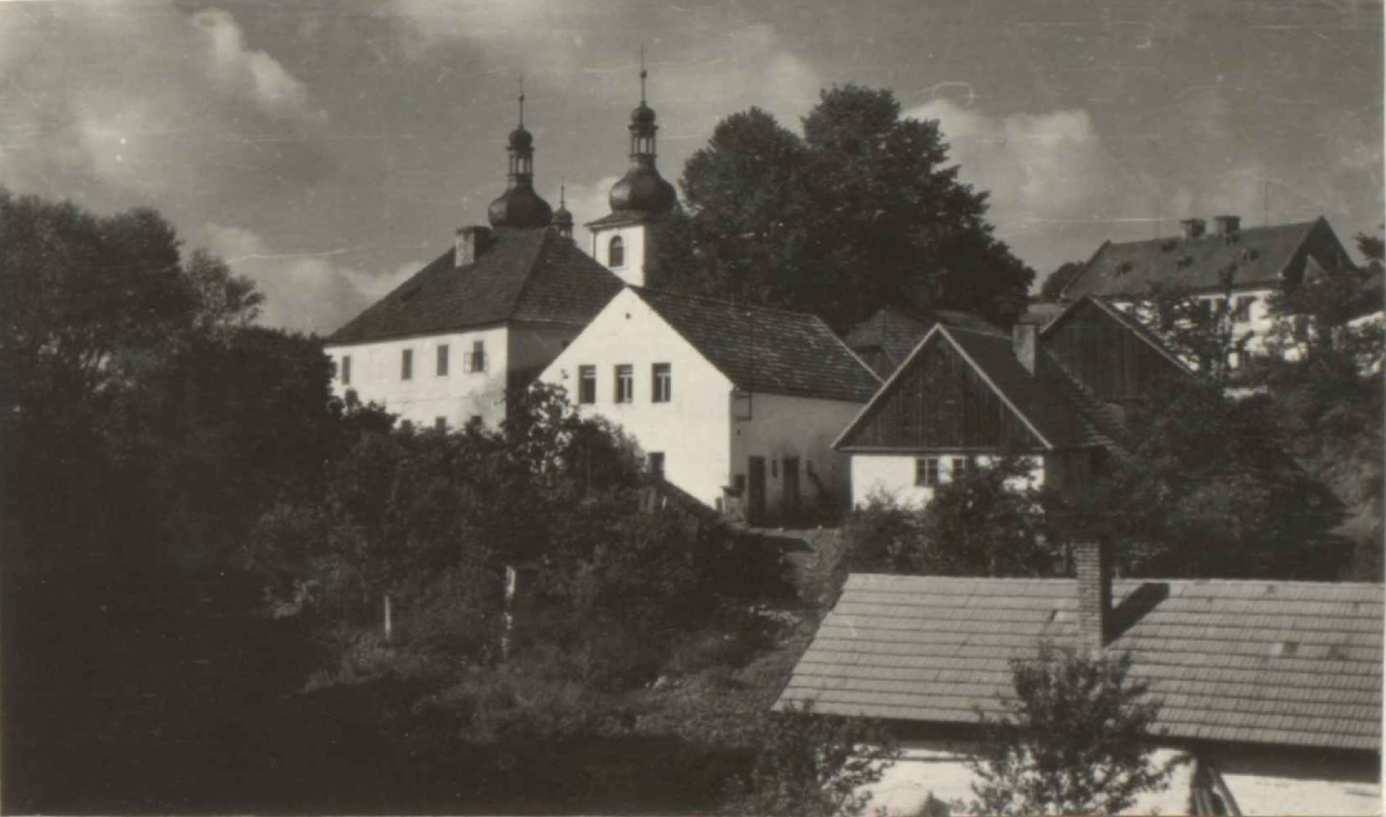
\includegraphics[width=\textwidth, height=\textheight, keepaspectratio]{241-a-straziste_u_mladotic}
\caption{Stražiště u Mladotic, sídlo rodové větve}
\label{fig:241-a-straziste_u_mladotic}
\end{figure}

             \begin{figure}
\centering
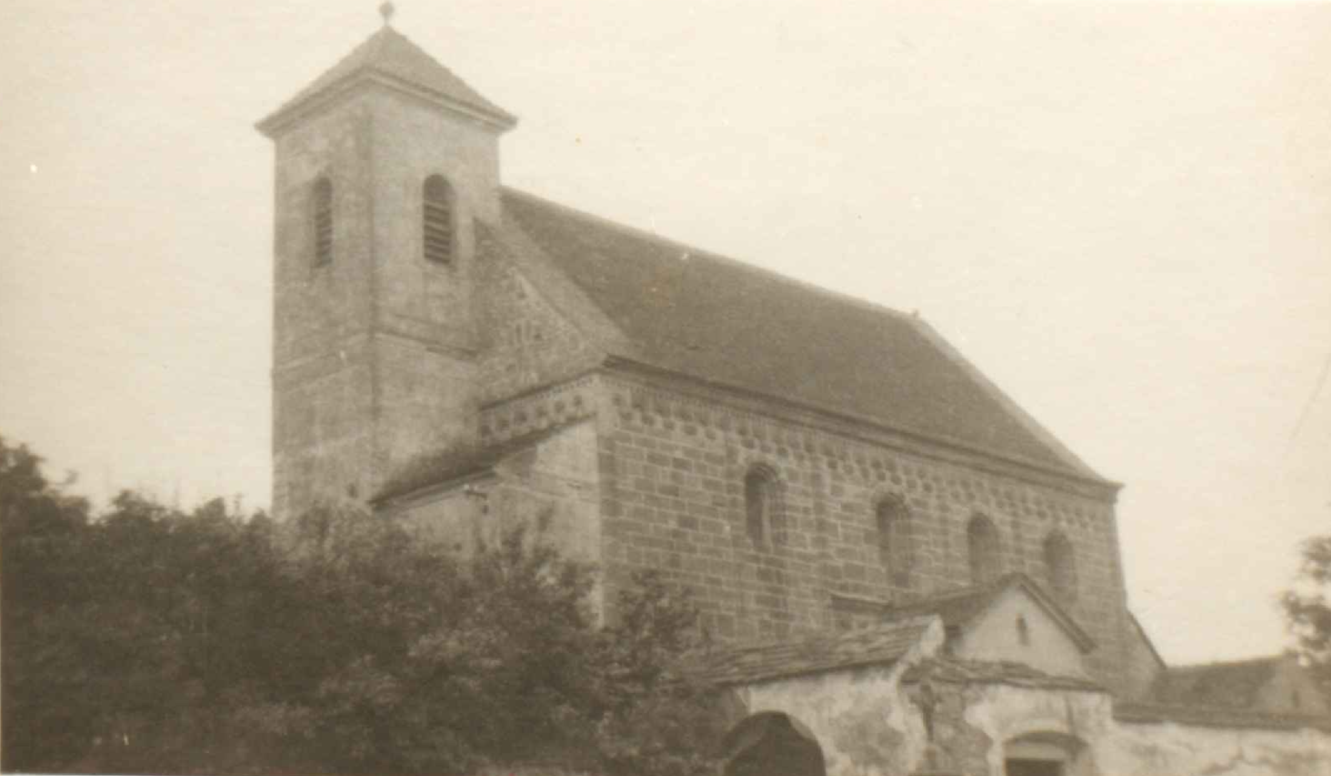
\includegraphics[width=\textwidth, height=\textheight, keepaspectratio]{241-b-kostel_v_potvorove}
\caption{Románský kostel svatého Mikuláše v Potvorově. Zde byli křtěni a pohřbíváni naši dávní předci}
\label{fig:241-b-kostel_v_potvorove}
\end{figure}


\end{document}
